\documentclass[a4paper]{article}

%% Language and font encodings
\usepackage[english]{babel}
\usepackage[utf8x]{inputenc}
\usepackage[T1]{fontenc}

%% Sets page size and margins
\usepackage[a4paper,top=3cm,bottom=2cm,left=3cm,right=3cm,marginparwidth=1.75cm]{geometry}

%% Useful packages
\usepackage{amsmath}
\usepackage{graphicx}
\usepackage[colorinlistoftodos]{todonotes}
\usepackage[colorlinks=true, allcolors=blue]{hyperref}

\title{Visma Homework Assignemnt for the Published Applications Solution Administrator Position}
\author{Edgar Ivanov}

\begin{document}
	\maketitle
	
	\section{Introduction}
	The task is to design infrastructure solution for the "Visma Services Norway". "Visma Services Norway" has approximately 1200 users using virtualized desktop environment and running its entire application portfolio in it. This document presents infrastructure solution and outlines the main design considerations.
	
	\section{Infrastructure Design}
	Figure \ref{fig:Diagram} presents the overall infrastructure design, followed by the design considerations for each FMA layer.
	
	\begin{figure}
		\centering
		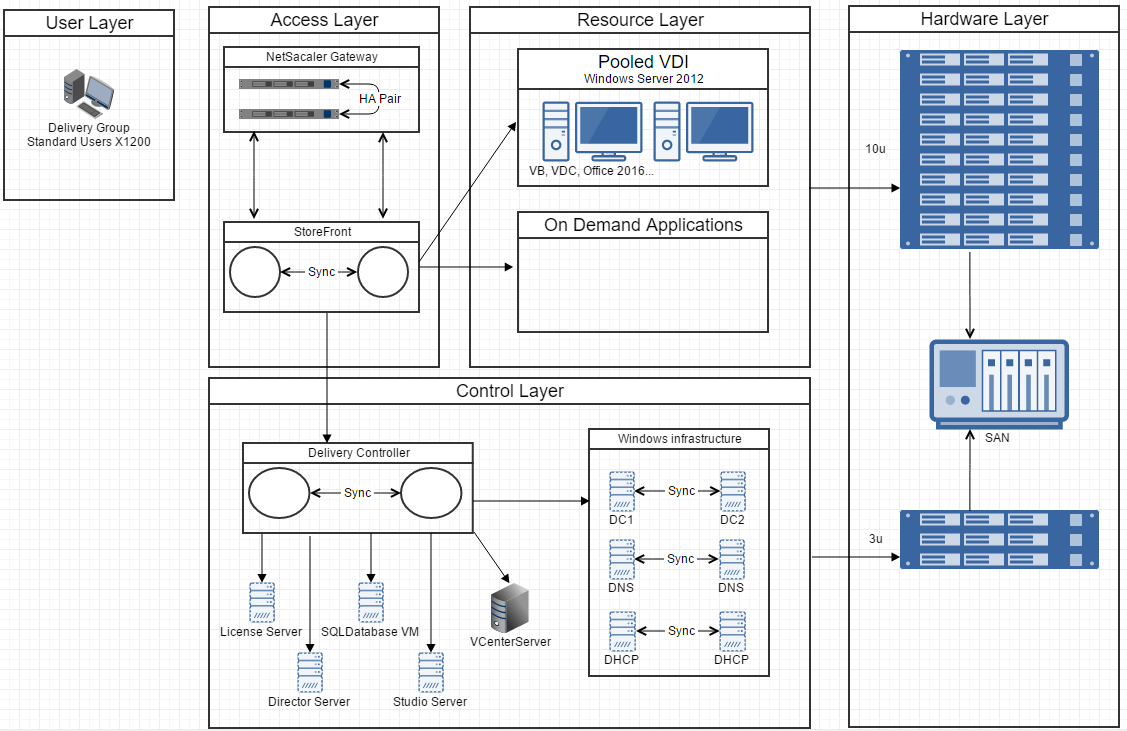
\includegraphics[width=1\textwidth]{InfrastructureDesign.png}
		\caption{\label{fig:Diagram}Infrastructure Design}
	\end{figure}
	
	\subsection{User Layer}
	User devices will require Citrix Receiver to be present and correctly configured in order to successfully access virtual desktop environment. Receiver can be deployed manually by the end users and auto configured with help of the auto provisioning file, initial deployment can also be done using GPOs or with help of any other third party solutions. Visma Services Norway (the client) is responsible for the endpoint device selection and management. The client should also have redundant internet line in order to eliminate connection issues.
	\subsection{Access Layer}
	To ensure high availability multi-active data centre deployment should be used. User base should be split in half, and redirected to the preferred site. Two VPX based NetScaler Gateways configured as HA pair should be deployed in the DMZ zone of each delivery site to isolate internal network from the outside world. All users will be treated as external users thus their connections will need to go through the NetScaler Gateway.
	
	Both data centres should have two StoreFront servers, first one accepting all connections and the second one in the stand by mode for the redundancy.  
	\subsection{Resource Layer}
	From the scenario we know that users will be connecting to the virtual desktops where they will be able launch applications, this leaves room only for the VDI environment either pooled  or personal . No specification is given whether users will be able to make any changes to their desktop, so we will assume that all desktops will be reset to the clean state after use. To facilitate application configuration persistence Citrix user profiles will be stored on the network share and loaded when user logs in.
	
	To provide resiliency at this layer VDI images should be stored on the networked storage, instead of the local, to eliminate image loss in case of the local disk failure. To ensure fast application provisioning all standard applications like MS Office, VB, VDC, Internet Browser should be pre-installed on the base image. Non standard applications may be streamed to the user Virtual Desktop in case there are special requirements.
	\subsection{Control Layer}
	All Windows components needed for the successfully application delivery, should be configured with the redundancies as well. There should be two domain controllers in each delivery site, two DNS servers as well as DHCP servers configured as a cluster.
	
	Delivery controller redundancy could be achieved by having at least two of them on the different physical hosts. Each Virtual Delivery Agent will be configured with the list of the available Delivery Controllers, thus providing redundancy in case of the Delivery Controller failure.
	
	Different techniques may be employed to achieve site database redundancy, including SQL mirroring, AlwaysOn Failover Clustering or AlwaysOn Availability Group. Having VMs running off the shared storage and servers configured in a cluster would allow the use of the VMware HA feature. With such setup virtual machine hosting SQL database and running on a clustered infrastructure would be automatically restarted on the different physical host in case of the original host failure. Further protection could be achieved by the use of the replication technology, where the copy of the machine would be stored in the different location, this would allow quick VM restoration as well.
	
	Licensing server may be left over as the built in 30-day grace period gives plenty of time for the service restoration.	
	\subsection{Hardware Layer}
	As per the original task we know that the hosting company utilizes SAN which most likely will be running in some king of the RAID configuration and providing redundancy at the storage level. All other components: network line, power supplies, server chassis should have spares ready for quick swap. Further hardware redundancy may be achieved with help of the VMware HA feature, which would bring up guest VMs from the failed host on to the healthy one.
	
	Hawing initial user count, their usage pattern and applications in use the following was identified as a requirement for the virtual desktops: each user would get a VM assigned with 2 vCPU cores, 2 GB of RAM and requiring 10 IOPS. Users will not be able to make any changes to the desktops, so the OS cache is not necessary. Golden image, with all applications preinstalled on it, shouldn't take more than 35 GB of storage space. Total storage required across two sites to accommodate all VMs for control layer and pooled desktops would be at around two terabytes.
	
	With numbers above in mind the following hardware would be required: eighteen servers with 192 GB of RAM and 20 CPU cores at 3 GHz each. No local storage is required except for the hypervisor which can perfectly run form the SD card. Two servers per data centre would be dedicated to the control layer VMs, while other seven servers would be dedicated to the VDI Pool. 	
	
	\section {Application Design}
	Figure \ref{fig:VismaWorkflow} presents the application work flow described in the provided scenario.
	\begin{figure}
		\centering
		\includegraphics[width=1.19\textwidth]{VismaWorkflow.png}
		\caption{\label{fig:VismaWorkflow}Application Workflow}
	\end{figure}

%	\href{https://www.citrix.com/blogs/2014/04/09/activeactive-gslb-for-xendesktop-a-practical-approach-part-1/}{Active/Active GSLB for XenDesktop}
	%\href{https://www.citrix.com/blogs/2012/11/24/xendesktop-high-availability-load-balancing-add-on-for-web-interface/}{XenDesktop – High Availability \& Load Balancing Add On For Web Interface}
\end{document}